\documentclass[11pt]{article}
\usepackage{geometry}                % See geometry.pdf to learn the layout options. There are lots.
\geometry{a4paper}                   % ... or a4paper or a5paper or ... 
%\geometry{landscape}                % Activate for for rotated page geometry
%\usepackage[parfill]{parskip}    % Activate to begin paragraphs with an empty line rather than an indent
\usepackage{graphicx}
\usepackage{amssymb}
\usepackage{epstopdf}
\DeclareGraphicsRule{.tif}{png}{.png}{`convert #1 `dirname #1`/`basename #1 .tif`.png}

\usepackage{hyperref}
\usepackage{textcomp}
\usepackage{xcolor}
\usepackage{underscore}
\usepackage{parskip}
\usepackage[nosolutionfiles]{answers}
\usepackage{tikz}
\usetikzlibrary{arrows,automata,shapes,snakes,patterns,decorations}
\usetikzlibrary{shapes.geometric,shapes.misc}
\usetikzlibrary{shadows}
\usetikzlibrary{calc}
\usetikzlibrary{positioning}
\usepackage{adjustbox}

\newcommand{\normaltilde}{{\raise.17ex\hbox{$\scriptstyle\mathtt{\sim}$}}}
\newcommand{\unixcl}[1]{\texttt{\fcolorbox{black}{gray!20}{#1}}}

\Newassociation{sol}{Solution}{ans}
\newtheorem{ex}{Question}


\title{Lab \#2\\$\star$\\Periodic tasks and Alarms}
\author{}
%\date{}                                           % Activate to display a given date or no date

\begin{document}
\maketitle

{\bf Note:} All the software and documents are stored at \url{http://www.irccyn.ec-nantes.fr/~bechenne/trampoline-isis}

\section{Goal}

Real-Time systems are reactive systems which have to do processing as a result of events. You have seen in Lab \#1 how to start processing as a result of an internal event of the system: by activating a task (\texttt{ActivateTask} and \texttt{ChainTask} services) or by setting an event (\texttt{SetEvent} service). In this lab, you will see how to trigger processing as a result of time passing (expiration of an Alarm). This lab uses the following concepts: alarm, counter. On the TP-ECN board, TIMER0 is used as interrupt source for alarms. The interrupt is sent every 1ms.

Go into the \texttt{trampoline/labs_isis/lab2} directory.

\section{First application}

\paragraph{lab2 application starting point} This application implements a periodic task that reads the push buttons of the board every 100ms.

Using the application of lab2 as a starting point, program an application which does a computation when a button is pushed. You will use a task named \texttt{t_process}, priority 3 that on odd execution displays ``processing triggered" and on even executions clears the LCD.

\section{Second application}

The second application will use 2 periodic tasks: \texttt{t1} (priority 2, period 1s) and \texttt{t2} (priority 1, period 1.5s). t1 toggles LED S0 each time it executes and t2 toggles LED S1.

\begin{ex}
Do not program directly. Give by hand the 20 first states of the LED given by the execution of the application with the display date of each state (0 being the application startup date). Is the whole system periodic ? If yes, what is the period and the behavior.
\end{ex}

\begin{ex}
The application needs a counter and 2 alarms. In Trampoline/ARM a counter is connected to a timer with a 1ms cycle time. What maximum \texttt{TICKSPERBASE} do you use to fulfill the application requirements ?
\end{ex}

\begin{ex}
How are the alarms configured to fulfill the application requirements ? Declare the counter and both alarms and write the application. Verify it works.
\end{ex}

\section{Third application}

In the third application, alarms, counters and polling on the push buttons are mixed. This application is a system with 2 push buttons. After starting the system waits. When the button is pressed, the system start a function F that is implemented using a periodic task (period = 1s). To ``see'' F, uses a blinking LED as in the second application. When the button is pressed again, function F is stopped. When the switch is pressed, the system is shutdown as quickly as possible (ie ShutdownOS is called).

\begin{ex}
Design and program this application using Trampoline.
\end{ex}

Requirements change. Now function F implementation needs an Init code
(runs once when the F is started) and a Final code (runs once when F is stopped).
This corresponds to the following diagram:

\begin{center}
\begin{adjustbox}{width=14cm,keepaspectratio}
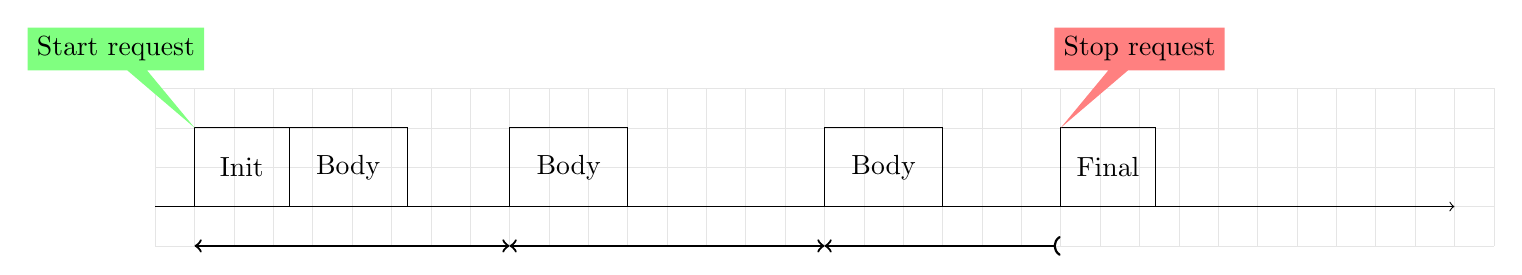
\begin{tikzpicture}
\draw[step=.5cm,gray!20,very thin] (-0.5, -0.5) grid (16.5,1.5);
\draw [->] (-0.5,0) -- (16,0);
\draw (0,0) rectangle (1.2,1);
\node at (0.6,0.5) {Init};
\draw (1.2,0) rectangle (2.7,1);
\node at (1.95,0.5) {Body};
\draw (4,0) rectangle (5.5,1);
\node at (4.75,0.5) {Body};
\draw (8,0) rectangle (9.5,1);
\node at (8.75,0.5) {Body};
\foreach \x in {0, 4}
  \draw [xshift=\x cm,thick,<->] (0,-0.5) -- (4,-0.5); 
\draw [xshift=8 cm,thick,<-(] (0,-0.5) -- (3,-0.5); 
\draw [xshift=11cm] (0,0) rectangle (1.2,1);
\node [xshift=11cm] at (0.6,0.5) {Final};
\node [rectangle callout, fill=green!50, callout absolute pointer={(0,1)}] at (-1,2) {Start request};
\node [rectangle callout, fill=red!50, callout absolute pointer={(11,1)}] at (12,2) {Stop request};
\end{tikzpicture}
\end{adjustbox}
\end{center}


\begin{ex}
Modify the application to take the new requirements into account. Use 3 basic tasks to implement function F. Init and Final print their names on the LCD.
\end{ex}

\begin{ex}
Same question but with only one extended task to implement function F.
\end{ex}

\section{Fourth application}

In this part, you will implement a watchdog. It is a mechanism that allows to stop a processing or the waiting for an event when a deadline occurs.

\begin{ex}
In your application, each time F0 is pressed, F1 must be pressed within 2 seconds. In such case, you print the time between the two occurrences. Otherwise, an error message is displayed. If 2 or more F0 are got within 3 seconds from the first one they are ignored.
\end{ex}

\begin{ex}
What is happening if the timeout occurs just after F1 has been pressed but before the waiting task got the event ? (draw a Gantt diagram of this scenario) If your application does not handle correctly this scenario, modify it.
\end{ex}

\section{Fifth application}

Program a chase\footnote{chenillard in French} with a 0.5s period. To do it, use 4 periodic tasks. Each periodic task manages a LED. The chase effect is done by using alarms with a time shift between them.

When F0 is pressed, the chase stops. When F1 is pressed, the chase continues. When F2 is pressed, the chase direction changes (even if it is stopped).

\end{document}  
